\documentclass[english]{beamer}%
%
\synctex=1
\usefonttheme{professionalfonts}
%
\usepackage{fontspec}%
\usepackage{amsmath,amsthm}%
\usepackage{unicode-math}
%\usepackage[mathcal]{euscript}%
\usepackage{stmaryrd}
\usepackage{polyglossia}
\usepackage{tikz,tikz-cd}
\usepackage{twoopt}
\usepackage{hyperref}
\usepackage{fmtcount}
\usepackage{microtype} % uncomment for better rendering
\usepackage{pdfrender}
\usepackage{prftree}
\usepackage{etoolbox}
\usepackage{pbox}
\usepackage{fontawesome}

\setmainlanguage{english}

\setmainfont{Linux Libertine O}[%
Ligatures={TeX,Rare,Historic,Common},%
Scale=MatchLowercase]%
\setsansfont{Roboto Light}[%
Scale=MatchLowercase,%
BoldFont=Roboto Medium,%
ItalicFont=Roboto Light Italic]%
\setmonofont{Ubuntu Mono}[Scale=MatchLowercase]%
\setmathfont{Libertinus Math Regular}%[Scale=MatchLowercase]%
\setmathfont{TeX Gyre Pagella Math}[range={\mathfrak,\rightleftarrows,\rightsquigarrow}]%
\setmathfont{DejaVu Math TeX Gyre}[range={\mathcal},Scale=MatchLowercase]%


\newfontfamily\custommathsffont{Lato Regular}[Scale=MatchLowercase,NFSSFamily=custommathsf]
\DeclareMathAlphabet{\mymathsf}{\encodingdefault}{custommathsf}{m}{n}

% macros are -*-latex-*- ones

%% macros about using categories
\DeclareMathOperator{\oboperator}{Ob}
\newcommand{\ob}[1]{\oboperator{#1}}
\DeclareMathOperator{\moroperator}{Mor}
\newcommand{\mor}[1]{\moroperator\left(#1\right)}
\newcommand{\op}[1]{{#1}^{\mathrm{op}}}
\newcommand{\comma}[2]{\left( #1 \mathbin{\downarrow} #2 \right)}
%\newcommand{\slice}[2]{\comma{#1}{#2}}
\newcommand{\slice}[2]{{#1}\kern-.5pt/\kern-1pt{#2}}
%\newcommand{\coslice}[2]{\comma{#2}{#1}}
\newcommand{\coslice}[2]{#2\kern-.5pt\backslash\kern-1pt#1}
\newcommand{\localize}[2]{{#2}^{-1}{#1}}
%\newcommand{\id}[1]{\mathrm{id}_{#1}}
\newcommand{\final}{1}
\newcommand{\initial}{0}
\newcommand{\psh}[1]{\widehat{#1}}
\DeclareMathOperator{\Pshoperator}{Psh}
\newcommand{\Psh}[1]{\Pshoperator(#1)}
\DeclareMathOperator{\Shoperator}{Sh}
\newcommand{\Sh}[1]{\Shoperator(#1)}
%\newcommand{\fiber}[2]{{#1}_{#2}}
\newcommand{\fiberprod}[3]{{#1}\times_{#3}{#2}}
\newcommand{\indout}[1]{\left\langle{#1}\right\rangle}
\newcommand{\indin}[1]{\left({#1}\right)}
\newcommand{\elemcat}[2][\null]{\int_{#1}{#2}}
\DeclareMathOperator*{\limoperator}{lim}
\renewcommand{\lim}[2][\null]{\limoperator_{#1}\left( #2 \right)}
\DeclareMathOperator*{\colimoperator}{colim}
\newcommand{\colim}[2][\null]{\colimoperator_{#1}\left( #2 \right)}
\newcommand{\limend}[1]{\int_{#1}}
\newcommand{\colimend}[1]{\int^{#1}}
\newcommand{\tens}{\mathbin \odot}
\newcommand{\cotens}{\mathbin \pitchfork}
%\newcommand{\adjoint}{\dashv}
\newcommand{\leftadjto}{\dashv}
\newcommand{\rightadjto}{\vdash}
\newcommand{\adjarrows}{\rightleftarrows}
\newcommand{\adjointarrows}{\rightleftarrows}
\newcommand{\ladjointmap}[2][]{{#2}_{#1}^\natural}
\newcommand{\radjointmap}[2][]{{#2}_{#1}^\flat}
\DeclareMathOperator{\spanoperator}{Span}
\newcommand{\catspan}[3][\null]{\spanoperator_{#1}\left(#2,#3\right)}
\DeclareMathOperator{\homoperator}{Hom}
% \renewcommand{\hom}[3][\null]{%
%         \ifx#1\null%
%                 \homoperator\left(#2,#3\right)%
%         \else #1\left(#2,#3\right) \fi}
\DeclareMathOperator{\Homoperator}{\underline{Hom}}
%\newcommand{\Hom}[3][\null]{\Homoperator_{#1}\left(#2,#3\right)}
\newcommand{\Arr}[1]{\operatorname{Arr}(#1)}
\DeclareMathOperator{\functorcatoperator}{Fun}
\DeclareMathOperator{\pseudofunctorcatoperator}{PFun}
\newcommand{\functorcat}[3][\null]{%
  \ifx#1\null%
  \functorcatoperator\left({#2},{#3}\right)%
  \else\Homoperator(#2,#3)%
  \fi%
}
\newcommand{\pseudofunctorcat}[3][\null]{%
  \ifx#1\null%
  \pseudofunctorcatoperator\left({#2},{#3}\right)%
  \else\Homoperator(#2,#3)%
  \fi%
}
\DeclareMathOperator{\opfiboperator}{OpFib}
\newcommand{\opfib}[1]{%
  \opfiboperator\left({#1}\right)%
}
\DeclareMathOperator{\bifiboperator}{BiFib}
\newcommand{\bifib}[1]{%
  \bifiboperator\left({#1}\right)%
}
\newcommand{\mono}{\hookrightarrow}
\newcommand{\epi}{\twoheadrightarrow}
\newcommand{\dom}{\mathrm{dom}}
\newcommand{\cod}{\mathrm{cod}}
\newcommand{\yoneda}[2][\null]{\mathfrak h^{#1}_{#2}}
\newcommand{\fromsum}[2]{\langle #1,#2 \rangle}
\newcommand{\toprod}[2]{\langle #1,#2 \rangle}
\newcommand{\inv}[1]{{#1}^{-1}}
\newcommand{\walkingcospan}{%
  \tikz[anchor=base,baseline,scale=.2]{%
    \draw[thick] (0,0) -| (1,1);%
  }%
}
\DeclareMathOperator{\nerveoperator}{N}
\newcommand{\nerve}[1]{\nerveoperator{#1}}

%% macros about bifibrational stuff
\DeclareMathOperator{\cartoperator}{Cart}
\newcommand{\cart}[3][\null]{\rho^{#1}_{#2,#3}}
\newcommand{\cartz}{\rho}
% \newcommand{\cart}[3][\null]{\cartoperator_{#1}\left(#2,#3\right)}
\DeclareMathOperator{\cocartoperator}{Cocart}
\newcommand{\cocart}[3][\null]{\lambda^{#1}_{#2,#3}}
\newcommand{\cocartz}{\lambda}
% \newcommand{\cocart}[3][\null]{\cocartoperator_{#1}\left(#2,#3\right)}
\newcommand{\push}[2]{{#1}_!#2}
\newcommand{\pull}[2]{{#1}^\ast#2}
\newcommand{\pushfact}[1]{{#1}_{\triangleright}}
\newcommand{\pullfact}[1]{{#1}^{\triangleleft}}
\newcommand{\middlefact}[3]{\vphantom{#1}_{#2}{#1}^{#3}}
\newcommand{\bigluing}[1]{\mathcal G\kern -.1em\ell\left(#1\right)}
\newcommand{\pseudo}[1]{\tilde{#1}}
\newcommand{\tensor}{\otimes}
\newcommand{\groth}[1]{\operatorname{\mathfrak{G}}({#1})}
\newcommand{\comp}[1]{\left\{#1\right\}}
\newcommand{\codtribe}[1]{\mathfrak p_{#1}}
\DeclareMathOperator{\subsetoperator}{Sub}
\newcommand{\Sub}[1]{\subsetoperator(#1)}

%% macros about Kan extensions
\newcommand{\restr}[1]{{#1}^\ast}
\newcommand{\lkan}[1]{{#1}_!}
\newcommand{\rkan}[1]{{#1}_\ast}

\newcommand*{\circled}[1]{\textrm{\textcircled{\small #1}}}

%% macros about formatting categories
\newcommand{\cat}[1]{\mathscr{#1}}
\newcommand{\concrete}[1]{\mymathsf{#1}}
% \newcommand{\Set}{\concrete{Set}}
% \newcommand{\Clan}{\concrete{Clan}}
% \newcommand{\RelClan}{\concrete{RelClan}}
% \newcommand{\Top}{\concrete{Top}}
% \newcommand{\Grpd}{\concrete{Grpd}}
% \newcommand{\Grp}{\concrete{Grp}}
% \newcommand{\Cat}{\concrete{Cat}}
% \newcommand{\Adj}{\concrete{Adj}}
% \newcommand{\Quil}{\concrete{Quil}}
% \newcommand{\Mod}{\concrete{Mod}}
% \newcommand{\CAT}{\concrete{CAT}}
% \newcommand{\Comp}{\concrete{Comp}}
% \newcommand{\sSet}{\boldsymbol{\cat S}}
\newcommand{\lincat}[1]{\mathbf{#1}}
\newcommand{\abgrp}[1]{{#1}_{\mathrm{ab}}}
\DeclareMathOperator{\lawthmodoperator}{Mod}
\newcommand{\lawthmod}[2][\null]{%
  \lawthmodoperator_{#2}
  \ifx#1\null%
  \null%
  \else%
  {\left(#1\right)}%
  \fi%
}
\newcommand{\finset}{\aleph_0}

%% simplicial stuff
\newcommand{\simpcat}{\boldsymbol\Delta}
\newcommand{\standsimp}[1]{\simpcat[#1]}
\newcommand{\simplicial}[1]{\boldsymbol{s}#1}
\newcommand{\face}[3][\null]{%
  \ifx#1\null%
  \partial_{#2}^{#3}%
  \else%
  \lexponent{\mathrm{d}_{#2}^{#3}}{#1}%
  \fi%
}
\newcommand{\degen}[3][\null]{%
  \ifx#1\null%
  \sigma_{#2}^{#3}%
  \else%
  \lexponent{\mathrm{s}_{#2}^{#3}}{#1}%
  \fi%
}

%% macros about model categories
\newcommand{\Ho}[2][\null]{\mathbf{Ho}_{\rm #1}\left( #2 \right)}
\newcommand{\class}[1]{\mathfrak{#1}}
\newcommand{\fib}{\mathrm{Fib}}
\newcommand{\cof}{\mathrm{Cof}}
%\newcommand{\weq}{\mathrm{W}}
\newcommand{\worth}[1][\null]{\mathbin{%
    \tikz[scale=.2,anchor=base,baseline]{%
      \draw (0,0) -- (1,0) -- (1,1) -- (0,1) -- (0,0) -- (1,1);%
    }_{#1}%
  }%
}%
\newcommand{\sorth}[1][\null]{
  \mathbin{\perp_{#1}}
}%
\newcommand{\bifibrant}[1]{{#1^{\rm cf}}}
\newcommand{\fibrant}[1]{{#1^{\rm f}}}
\newcommand{\cofibrant}[1]{{#1^{\rm c}}}
\newcommand{\fibrantrep}[1]{\mathfrak j_{#1}}
\newcommand{\cofibrantrep}[1]{\mathfrak q_{#1}}
\newcommand{\fibrantrepz}{\fibrantrep\null}
\newcommand{\cofibrantrepz}{\cofibrantrep\null}
\DeclareMathOperator*{\lderivoperator}{\mathbf L}
\DeclareMathOperator*{\rderivoperator}{\mathbf R}
\newcommand{\lderiv}[1]{\lderivoperator#1}
\newcommand{\rderiv}[1]{\rderivoperator#1}
\newcommand{\htpyclass}[1]{\left[ #1 \right]}
\newcommand{\htpyhom}[3][\null]{\pi\left(#2,#3\right)_{#1}}
\newcommand{\htpyquotient}[1]{\pi\,{#1}}
% \newcommand{\htpyhom}[3][\null]{\left[ #2,#3 \right]_{#1}}
\DeclareMathOperator*{\derivfwoperator}{\mathbf D}
\newcommand{\derivfw}[1]{\derivfwoperator{#1}}
\newcommand{\disc}[1]{#1_{\rm d}}
%\newcommand{\triv}[1]{#1_{\rm triv}}
\newcommand{\fiberwise}[1]{#1_{\rm fw}}
\newcommand{\lexponent}[2]{\vphantom{#1}^{#2}{#1}}
\newcommand{\llp}[1]{\lexponent{#1}{\worth}}
\newcommand{\rlp}[1]{{#1}^{\worth}}
\newcommand{\wllp}[2][\null]{\lexponent{#2}{\worth[#1]}}
\newcommand{\wrlp}[2][\null]{{#2}^{\worth[#1]}}
\newcommand{\sllp}[2][\null]{\lexponent{#2}{\sorth[#1]}}
\newcommand{\srlp}[2][\null]{{#2}^{\sorth[#1]}}
\newcommand{\lhmtp}{\mathrel{\sim_\ell}}
\newcommand{\rhmtp}{\mathrel{\sim_r}}
\newcommand{\hmtp}{\mathrel{\sim}}
\newcommand{\iso}{\cong}
\newcommand{\htpyeq}{\simeq}

%% macros dealing with Reedy stuff
\newcommand{\deginf}[2]{#1_{#2}}
\DeclareMathOperator{\latchingoperator}{L}
\newcommand{\latch}{\latchingoperator}
\newcommand{\latching}[1]{\latchingoperator_{#1}}
\DeclareMathOperator{\matchingoperator}{M}
\newcommand{\match}{\matchingoperator}
\newcommand{\matching}[1]{\matchingoperator_{#1}}

%% macros about set-theoretic stuff
\newcommand{\universe}[1]{\mathbb{#1}}
\newcommand{\powerset}[1]{\operatorname{\mathcal P}\left(#1\right)}

%% macros about type theoretic stuff
\newcommand{\theory}[1]{\mathbb{#1}}
\newcommand{\Var}{\mymathsf{Var}}
\newcommand{\entails}{\mathrel{\vdash}}
\newcommand{\defequal}{\mathrel{\equiv}}
\newcommand{\type}[1]{{#1}\ \mymathsf{type}}
\newcommand{\ctxt}[1]{{#1}\ \mymathsf{context}}
\newcommand{\subs}[3]{{#1}\left[#2\!\gets\!#3\right]}
\newcommand{\freevar}[1]{\mymathsf{fv}\left(#1\right)}
\newcommand{\alphabet}[1]{\mathcal{#1}}
\newcommand{\shift}[2][\null]{\mymathsf{pr}_{#2}^{#1}}
\newcommand{\var}{\mathrm{var}}
\newcommand{\idsymbol}{\mathrm{Id}}
\newcommand{\eqsymbol}{\mathrm{Eq}}
\newcommand{\sumsymbol}{\Sigma}
\newcommand{\prodsymbol}{\Pi}
\newcommand{\sumtype}[2]{\sumsymbol_{#1}#2}
\newcommand{\prodtype}[2]{\prodsymbol_{#1}#2}
\newcommand{\locprod}[2]{\prodsymbol_{#1}{#2}}
\newcommand{\idtype}[3][\null]{\operatorname{\idsymbol}_{#1}\left(#2,#3\right)}
\newcommand{\eqtype}[3][\null]{\operatorname{\eqsymbol}_{#1}\left(#2,#3\right)}
%\newcommand{\refl}[1]{\mymathsf{refl}_{#1}}
\newcommand{\jidoperator}{\mymathsf{j}}
\newcommand{\jid}[4]{\jidoperator(#1,#2,#3,#4)}
\newcommand{\transid}[2]{\mymathsf{trans}_{#1}\ifx#2\null\null\else(#2)\fi}
\newcommand{\name}[1]{\ulcorner{#1}\urcorner}
\newcommand{\recnat}[1]{\ifx#1\null\mymathsf{rec}\else\mymathsf{rec}(#1)\fi}
\newcommand{\sing}[1]{\mymathsf{isContr}(#1)}
\newcommand{\hequiv}[1]{\mymathsf{isEquiv}(#1)}
\newcommand{\idisequiv}[1]{\mymathsf{idIsEquiv}_{#1}}
\newcommand{\idtoeq}{\mymathsf{IdtoEq}}
\newcommand{\rewrite}[1][\null]{\mathrel{\rightsquigarrow}_{#1}}
%% semantics
\newcommand{\sem}[1]{\llbracket#1\rrbracket}
\newcommand{\domsem}[1]{\sem{#1}_0}
\newcommand{\codsem}[1]{\sem{#1}_1}
\newcommand{\loctribe}[2]{{#1}\,(#2)}
\newcommand{\locreltribe}[3]{\mathrm P_{#3}{#1}\,(#2)}

%% macros about general math
\DeclareMathOperator{\autoperator}{Aut}
%\newcommand{\aut}[1]{\autoperator\left(#1\right)}
\newcommand{\quotient}[2]{\left. {#1} \middle / {#2} \right.}
\newcommand*\from{:}
\newcommand*\cocolon{%
  \nobreak
  \mskip6mu plus1mu
  \mathpunct{}%
  \nonscript
  \mkern-\thinmuskip
  {:}%
  \mskip2mu
  \relax
}
\newcommand*\cofrom{:}
\DeclareMathOperator{\im}{im}
\newcommand{\blank}{\mathord{\color{lightgray}-}}
\newcommand{\Naturals}{\mathbb{N}}
%\newcommand{\doteq}[1][]{\mathrel{\cdot=_{#1}}}

%% macros about general typesetting
\newcommand{\define}[1]{\emph{#1}}
\newcommand{\showcase}[1]{\textbf{#1}}
\newcommand{\nb}[1]{\nobreakdash#1}

\newcommand{\mltt}{{\sc mltt}}%
\newcommand{\wfs}{\textsc{wfs}}

%% theorems typesetting
\newtheorem{theorem}{Theorem}[section]
\newtheorem*{theorem*}{Theorem}
\newtheorem*{theorem_french*}{Théorème}
\newtheorem{proposition}[theorem]{Proposition}
\newtheorem*{proposition*}{Proposition}
\newtheorem{lemma}[theorem]{Lemma}
\newtheorem{corollary}[theorem]{Corollary}
\newtheorem{claim}[theorem]{Claim}
\newtheorem*{claim*}{Claim}
\theoremstyle{definition}
\newtheorem{definition}[theorem]{Definition}
\newtheorem*{definition*}{Definition}
\newtheorem*{definition_french*}{Définition}
\newtheorem{defprop}[theorem]{Definition-Proposition}
\theoremstyle{remark}
\newtheorem{remark}[theorem]{\sc Remark}
\newtheorem{notation}[theorem]{\sc Notation}
\newtheorem{vocabulary}[theorem]{\sc Terminology}
\newtheorem{example}[theorem]{\sc Example(s)}
\newtheorem{cexample}[theorem]{\sc Counterexample(s)}
%
%% to get the correct cleveref functionality
%% we redefine the thm enviroments from lmcs.cls
\newcommand{\renewtheorem}[1]{%
  \expandafter\let\csname #1\endcsname\relax
  \expandafter\let\csname c@#1\endcsname\relax
  \expandafter\let\csname end#1\endcsname\relax
  \newtheorem{#1}%
}

\theoremstyle{plain}

\renewtheorem{thm}{Theorem}[section]
\crefname{thm}{Theorem}{Theorems}
\renewtheorem{cor}[thm]{Corollary}
\crefname{cor}{Corollary}{Corollaries}
\renewtheorem{lem}[thm]{Lemma}
\crefname{lem}{Lemma}{Lemmas}
\renewtheorem{prop}[thm]{Proposition}
\crefname{prop}{Proposition}{Propositions}

\theoremstyle{definition}

\renewtheorem{rem}[thm]{Remark}
\crefname{rem}{Remark}{Remarks}
\renewtheorem{exa}[thm]{Example}
\crefname{exa}{Example}{Examples}
\renewtheorem{defi}[thm]{Definition}
\crefname{defi}{Definition}{Definitions}

% Meta-macros for:
\newcommand*{\constant}[1]{\mathrm{#1}}% defined constants : roman
\newcommand*{\constructor}[1]{\mathrm{#1}} % constructors : italic
\newcommand*{\typeformer}[1]{\mathrm{#1}} % (uppercase) typeformers : roman

%% Macros
\let\oldequiv\equiv

\renewcommand*{\th}{\textsuperscript{th}}
\newcommand*{\from}{:}
\newcommand*{\blank}{\mathord{{-}}}%{\color{lightgray}-}}
\newcommand*{\inv}[1]{#1^{-1}}

\newcommand*{\set}[1]{\{#1\}}
\newcommand*{\refl}[1]{\mathop{{\constructor{refl}}_{#1}}}
\newcommand*{\refloi}[1]{\mathop{\constructor{refl}^{-o}_{#1}}}
\newcommand*{\inl}{\mathop{\constructor{inl}}}
\newcommand*{\inr}{\mathop{\constructor{inr}}}
\newcommand*{\mrd}{\operatorname{\constructor{mrd}}}
\newcommand*{\glue}{\operatorname{\constructor{glue}}}
\newcommand*{\north}{\constructor{N}}
\newcommand*{\south}{\constructor{S}}
\newcommand*{\trp}[2][]{\mathop{\constant{trp}^{#1}_{#2}}}
\newcommand*{\fst}{\mathop{\constant{fst}}}
\newcommand*{\snd}{\mathop{\constant{snd}}}
\newcommand*{\funext}{\mathop{\constant{funext}}}
\newcommand*{\ptw}{\mathop{\constant{ptw}}}
\newcommand*{\ap}[1]{\mathop{\left[{#1}\right]}}
\newcommand*{\ptdto}{\to_\ast}%
\newcommand*{\ptdweq}{\weq_\ast}%
\newcommand*{\loopspace}[1]{\mathop{\Omega^{#1}}}%

\newcommand*{\nat}{\mathord{\constant{nat}}}
\newcommand*{\ltr}{\mathord{\constant{ltr}}}
\newcommand*{\rtr}{\mathord{\constant{rtr}}}

\newcommand*{\Id}{\mathord{\constant{Id}}}
\newcommand*{\id}{\mathord{\constant{id}}}
\newcommand*{\cat}[1]{\mathscr{#1}}

\newcommand*{\weq}{\simeq}
\newcommand*{\QQ}{\mathbb{Q}}
\newcommand*{\ZZ}{\mathbb{Z}}
\newcommand*{\NN}{\mathbb{N}}
\newcommand*{\CC}{\mathbb{C}}
\newcommand*{\RR}{\mathbb{R}}
\newcommand*{\isom}{\cong}
\newcommand*{\ct}{*}
\newcommand*{\cto}{*_{\mathrm{o}}}

%\renewcommand{\equiv}{\simeq}
%\newcommand*{\liff}{\equiv}
\newcommand*{\jdeq}{\equiv}
%\newcommand*{\defeq}{\mathrel{\hbox{:}\mkern-5mu\equiv}}
\newcommand*{\defeq}{\vcentcolon\jdeq}
\newcommand*{\defequi}{\defeq}%definitionally equal}
\newcommand*{\defis}{\vcentcolon=}
% \newcommand*{\defis}{\mathrel{\hbox{:}\mkern-5mu=}}
\newcommand*{\leftadjto}{\dashv}

\DeclareMathOperator\im{im}
\DeclareMathOperator\Aut{Aut}

\DeclarePairedDelimiter\Trunc{\lVert}{\rVert}
\DeclarePairedDelimiter\trunc{\lvert}{\rvert} % truncation
\DeclarePairedDelimiter\angled{\langle}{\rangle}
\DeclarePairedDelimiterX\setof[2]\lbrace\rbrace{#1 \mid #2}

\newcommand*{\nonempty}[1]{\Trunc{#1}}
\newcommand*{\setTrunc}[1]{\Trunc{#1}_0}
\newcommand*{\settrunc}[1]{\trunc{#1}_0}

\DeclarePairedDelimiterXPP\higherTrunc[2]{}\lVert\rVert{_{#1}}{#2}
\DeclarePairedDelimiterXPP\highertrunc[2]{}\lvert\rvert{_{#1}}{#2}

\newcommand*{\merely}[1]{\higherTrunc{-1}{#1}}

%%%%%%%%%%%%%%%%%%%%%%%%%%%%%%%%%%%%%%%%%%%%%%%%%%%%%%%%%%%%%%%%%%%%%%%%%%%%
\newcommand*{\ev}{\constant{ev}}
\newcommand*{\ve}{\constant{ve}}
\newcommand*{\el}{\constant{elim}}

\newcommand*{\iscontr}{\constant{isContr}}
\newcommand*{\isprop}{\constant{isProp}}
\newcommand*{\isset}{\constant{isSet}}
\newcommand*{\isgrpd}{\constant{isGrpd}}
\newcommand*{\isequiv}{\constant{isEquiv}}
\newcommand*{\isonetype}{\constant{1Type}}
\newcommand*{\isconn}{\constant{isConn}}
\newcommand*{\istrunc}[1]{\constant{isTrunc}_{#1}}

\newcommand*{\conncomp}[2]{{#1}_{\left(#2\right)}}

\newcommand*{\UU}{\mathcal{U}}
\newcommand*{\UUp}{\UU_*}
\newcommand*{\UUptd}{\UUp}
\newcommand*{\pttype}{\UUp}

\newcommand*{\circled}[1]{\textrm{\textcircled{\small #1}}}

\newcommand*{\hopf}{{\mathcal H}}
\newcommand*{\Sn}[1]{{\mathbb S^{#1}}}% general sphere
\newcommand*{\Sc}{{\Sn 1}}%the circle
\newcommand*{\Sp}{{\Sn 2}}%the 2-sphere
\newcommand*{\sbt}{\tikz[baseline]{\node[scale=.7,inner
    sep=0, outer sep=0, circle, anchor=base, yshift=.05ex]%
    {$\bullet$};}}%
\newcommand*{\base}{\mathord{\sbt}}%point in circle
\newcommand*{\uc}[1]{{I_{#1}}}%universal set bundle
\newcommand*{\Sloop}{\mathord{\circlearrowleft}}%loop in circle
\newcommand*{\bn}[1]{\mathbf{#1}}
\newcommand*{\emptytype}{\emptyset}
\newcommand*{\ind}{\operatorname{\constant{ind}}}
\newcommand*{\susp}{\operatorname{\Sigma}}
\newcommand*{\hcomp}{\mathbin{\cdot}} % was : \cdot_h

\newcommand*{\etop}[1]{\bar {#1}}
\newcommand*{\ptoe}[1]{\tilde {#1}}

%% fundamental group
\newcommand*{\hgr}[1]{\uppi_{#1}}
\newcommand*{\fgr}{\hgr 1}

%% paths over paths

%% \newcommand*{\pathover}[4]{#1 \overset{#2}{\underset{#3}=} #4}
\newcommand*{\pathoverdisplay}[4]{{#1} \overset{#2}{\underset{#3}=} #4}
\newcommand*{\pathover}[4]{#1 =^{#2}_{#3} #4}

%% global tikz styles
\usetikzlibrary{arrows}

\tikzset{cell/.style={%
    shorten <=1em,%
    shorten >=1em,
    /tikz/commutative diagrams/Rightarrow
  }%
}%
\tikzset{
tikzshortarrow/.style={
    shorten >=0.2cm,
    shorten <=0.2cm,
    thick,
  }
}
\tikzset{pushout/.style={%
    commutative diagrams/.cd,dr,phantom,"\ulcorner", very near end
  }%
}
\tikzset{
    rotninety/.style={anchor=south, rotate=90, inner sep=2pt}
}
\tikzset{
    rottwoseventy/.style={anchor=north, rotate=90, inner sep=2pt}
}

\definecolor{darkgreen}{rgb}{0,0.4,0}
\definecolor{darkblue}{rgb}{0,0,1}
\definecolor{darkred}{rgb}{.7,0,0}

\tikzset{
	tikzforeground/.style={
		->,
%		shorten >=0.2cm,
%		shorten <=0.2cm,
		line width = 0.8pt,
		preaction={draw, -, line width=5pt, white},
	},
	tikzbackground/.style={
		->,
%		shorten >=0.2cm,
%		shorten <=0.2cm,
		line width = 0.4pt,
	},
%	tikzmiddle/.style={
%		->,
%		shorten >=0.2cm,
%		shorten <=0.2cm,
%		line width = .8pt,
%		preaction={draw, -, line width=3pt, white},
%	},
	tikzequal/.style={
		-,
		double,
		shorten >=0.2cm,
		shorten <=0.2cm,
		line width = 0.6pt,
		preaction={draw, -, line width=3pt, white},
	},
}
%
\newcommand{\susp}{\Sigma}%
\newcommand{\ptdto}{\to_\ast}%
\newcommand{\hopffam}{\mathcal H}%


\usetikzlibrary{decorations.pathmorphing}
\usetikzlibrary{decorations.markings}
\usetikzlibrary{calc,3d}
\usetikzlibrary{arrows,shapes,decorations.pathreplacing}


\makeatletter
% Insert [short title] for \section in ToC
\patchcmd{\beamer@section}{{#2}{\the\c@page}}{{#1}{\the\c@page}}{}{}
\makeatother
\setbeamertemplate{section page}{%
  %\begin{frame}
    % \vfill
    % % 
    % \centering \usebeamercolor[fg]{structure}{%
    % \huge \tikz{\node[draw=fg,thick,circle] {\arabic{section}};}
    % \\[30pt] % \hskip 10pt %
    % \secname}
    % % 
    % \vfill
    \begin{tikzpicture}[remember picture, overlay]
      % \node[anchor=west,outer sep=0pt,inner sep=0pt] (number) at
      % ([xshift=20pt]current page.west) {%
      % \itshape \Large \color{structure.fg} \arabic{section}};%
      % \node[anchor=west] (point) at ([xshift=-2pt,yshift=-3pt]
      % number.east) {%
      % \itshape \huge \color{structure.fg} .};%
      \node[anchor=west] (name) at ([xshift=20pt,yshift=-2pt] current
      page.west) {%
        \Large \color{structure.fg} \arabic{section}. \hskip 3pt
        \secname%
      };%
      \path ([xshift=5pt] name.east) coordinate (start) -| coordinate
      (stop) ([xshift=-20pt] current page.east);%
      \draw[orange,line width=.1pt,rounded corners]
      ([xshift=-50pt,yshift=-5pt] name.south east) -| (start) --
      (stop);%
    \end{tikzpicture}
 % \end{frame}%
}

\makeatletter
\newcommand{\logouniv}[1]{\def\@logouniv{#1}}%
\newcommand{\logolab}[2][10mm]{\def\@logolabh{#1}\def\@logolab{#2}}%
\newcommand{\logoother}[1]{\def\@logoother{#1}}%
\makeatother

\title{Symmetries of $\mathbb S^n$}%
\subtitle{%
  \footnotesize in univalent foundations%
}%
\author{Pierre Cagne\\
  {\normalsize (joint work with Nicolai Kraus and Marc Bezem)}%
}%
\institute{Universitetet i Bergen}
\date{TYPES 2020 -- Turin\\ March ??, 2020%
}%
\logouniv{UiBlogoMN_gray_v.png}%
% \logolab[7mm]{}%
% \logoother{}%

\setbeamertemplate{section in toc}[sections numbered]
\setbeamertemplate{itemize items}[star]


% \makeatother
% \setbeamertemplate{headline}
% {%
%   \vskip5pt \hfill \color{lightgray} \bfseries%
%   \insertframenumber{} / \inserttotalframenumber\hspace*{1em}%
%   \vskip0pt%
% }
\makeatletter
\addtobeamertemplate{background}{}{%
  \ifnum\c@framenumber=1%
  \else%
  \begin{tikzpicture}[remember picture,overlay]
    % \coordinate [xshift=-2em,yshift=-2em] (P) at (current page.north
    % east) {};% {\color{structure.fg!60} \insertframenumber};%
    % \fill[structure.fg!20,line width=3pt] (P) ++ (0,2/5) arc
    % (90:90+360:2/5);%
    % \fill[structure.fg!60] (P) to (P) ++ (0,2/5) arc
    % (90:90+360*\insertframenumber/\inserttotalframenumber:2/5) to (P)
    % ;%
    \coordinate[yshift=-3em] (start) at (current page.north west);%
    \coordinate[yshift=-3em] (stop) at (current page.north east);%
    \path let \p1 = (start), \p2 = (stop) in
    ([xshift=(\x2-\x1)*(\insertframenumber/\inserttotalframenumber)]
    start) coordinate (curr);%
    \draw[orange!20,line width=.1pt] (start) -- (stop);%
    \draw[orange,line width=.1pt] (start) -- (curr);%
    \fill[orange] (curr) circle (1pt);
  \end{tikzpicture}%
  \fi%
}
\makeatother

\setbeamertemplate{navigation symbols}{}

\tikzset{%
  mid arrow/.style={%
    postaction={decorate,%
      decoration={
        markings,
        mark=at position .5 with {\arrow[#1]{stealth}}
      }%
    }%
  }%
}

\tikzset{ampersand replacement=\&}

\tikzset{onslide/.code args={<#1>#2}{%
    \only<#1>{\pgfkeysalso{#2}} 
  }%
}

\tikzset{
  invisible/.style={opacity=0,text opacity=0},
  visible on/.style={alt={#1{}{invisible}}},
  alt/.code args={<#1>#2#3}{%
    \alt<#1>{\pgfkeysalso{#2}}{\pgfkeysalso{#3}}%
  }%
}

\tikzset{%
  popup/.style args={color=#1}%
  {fill=#1!20,rounded corners=5,draw=#1!80,line width=1pt,inner
    sep=5pt},%
  babypopup/.style args={color=#1}%
  {fill=#1!20,rounded corners=5,inner sep=3pt},%
  popuparr/.style args={color=#1}%
  {->,#1!80,line width=3pt,>=stealth}%
}

\tikzset{%
  pathdec/.style={%
    decoration={%
      markings,%
      mark=at position .5 with {%
        \arrow[black]{>};%
      }%
    }%
    ,postaction=decorate%
  }%
}

\makeatletter
\setbeamertemplate{title page}{%
  \colorlet{titlecolor}{structure.fg}
  \begin{tikzpicture}[remember picture,overlay]%
    % \coordinate (aux1) at ([xshift=5pt]
    % current page.north west); %
    % \coordinate (aux2) at ([xshift=200pt]current page.north west); 
    % % \coordinate (aux3) at ([yshift=-4cm]current page.north west); 
    % \coordinate (aux4) at ([xshift=70pt]current page.north west);

    % \begin{scope}[titlecolor!40,line width=6pt,scale=.6]
    %   \draw (aux1) arc (200:340:3.5) coordinate[midway] (a) coordinate
    %   (b);%
    %   \draw (a) arc(-20:-110:3);
    %   \draw[opacity=0.6,titlecolor]
    %   (b) arc (200:340:2.5) coordinate (bb);
    %   \draw[titlecolor,line width=3pt,rounded corners=4pt]
    %   (aux4) arc (190:350:1);
    % \end{scope}
    % \begin{scope}[titlecolor!70,line width=2pt,rounded
    %   corners=4pt,scale=.5]%
    %   \draw ([xshift=125pt] bb) arc (200:340:2.6) coordinate[near start]
    %   (c) ;%
    %   \draw (c) arc (-45:-160:1.7) coordinate (d);%
    %   \draw (d) arc (-45:10:1.1); \draw (d) arc (-45:-170:1.1);%
    % \end{scope}
    %%
    % \fill[structure!80] ([yshift=30pt]current page.west) rectangle
    % ([yshift=20pt]current page.south east);%
    %
    %%% logos
    \coordinate (logouniv_xy) at
    ([xshift=\marginparsep,yshift=-\marginparsep] current page.north
    west);%
    \node [anchor=north west] (logouniv) at (logouniv_xy) {%
      \ifx\@logouniv\undefined%
      \null%
      \else {\includegraphics[height=10mm]{\@logouniv}}%
      \fi%
    };%
    %
    % \draw[very thin] ([yshift=-10pt]logouniv.north east) --
    % ([yshift=10pt]logouniv.south east);
    %
    \def\loglabh{\ifx\@logolabh\undefined 0\else\@logolabh\fi}%
    \coordinate (logolab_xy) at
    ([xshift=7pt,yshift=-((10mm-\loglabh)/2)] logouniv.north east);%
    \node [anchor=north west] (logolab) at (logolab_xy) {%
      \ifx\@logolab\undefined%
      \null%
      \else {\includegraphics[height=\@logolabh]{\@logolab}}%
      \fi%
    };%
    %
    \coordinate (logoother_xy) at
    ([xshift=\marginparsep,yshift=\marginparsep] current page.south
    west);%
    \node [anchor=south west] (logoother) at (logoother_xy) {%
      \ifx\@logoother\undefined%
      \null%
      \else {\includegraphics[height=10mm]{\@logoother}}%
      \fi%
    };%
    %%%%
    \node[anchor=east] at ([yshift=-60pt,xshift=-20pt]current
    page.north east) (author) {%
      \parbox[t]{.6\paperwidth}{\raggedleft%
        \usebeamerfont{author}\textcolor{structure.fg}{%
          \textpdfrender{ TextRenderingMode=FillStroke,
            FillColor=structure.fg, LineWidth=.05ex,}
          {\large\insertauthor}%
        }%
      }%
    };%
    %%%%
    \node[anchor=north west] at
    (author.south west)
    (institute) {%
      \parbox[t]{.6\paperwidth}{\raggedleft%
        \usebeamerfont{institute}%
        \textcolor{gray}{\insertinstitute}%
      }%
    };%
    % \node[anchor=west,opacity=.8] at
    % ([yshift=-10pt,xshift=20pt]current page.west) (logo) {%
    %   \parbox[t]{.19\paperwidth}{\raggedleft%
    %     \usebeamercolor[structure.fg]{titlegraphic}\inserttitlegraphic%
    %   }%
    % };%
    \node[anchor=center] at ([yshift=-1em,xshift=0pt]current
    page.center) (title) {%
      \parbox[t]{.5\textwidth}{\centering%
        \usebeamerfont{title}\textcolor{structure.fg}{%
          \textpdfrender{ TextRenderingMode=FillStroke,
            FillColor=structure.fg, LineWidth=.05ex, }{%
            \huge\inserttitle%
          }%
          \\
          \usebeamerfont{subtitle}\Large\insertsubtitle%
        }%
      }%
    };%
    \draw[orange,line width=.1pt,rounded corners]
    ([yshift=-15pt,xshift=-15pt] title.north west) coordinate (start)
    |- ([yshift=20pt,xshift=50pt] title.north west);%
    \draw[orange,line width=.1pt,rounded corners]
    ([yshift=5pt,xshift=15pt]title.south east) coordinate (end) |-
    ([yshift=-20pt,xshift=-120pt] title.south east);%
    \fill[orange!70] (start) circle (1pt);%
    \fill[orange!70] (end) circle (1pt);%
    %%%
    \node[anchor=north west] at
    ([yshift=-50pt,xshift=0pt]title.south)
    (date) {%
      \parbox[t]{.4\paperwidth}{\raggedleft%
        \usebeamerfont{date}%
        \textcolor{orange}\insertdate%
      }%
    };%
    \node[anchor=center,opacity=.1] at
    %([yshift=0pt,xshift=150pt]current page.west)%
    (current page.center)%
    (pic) {%
        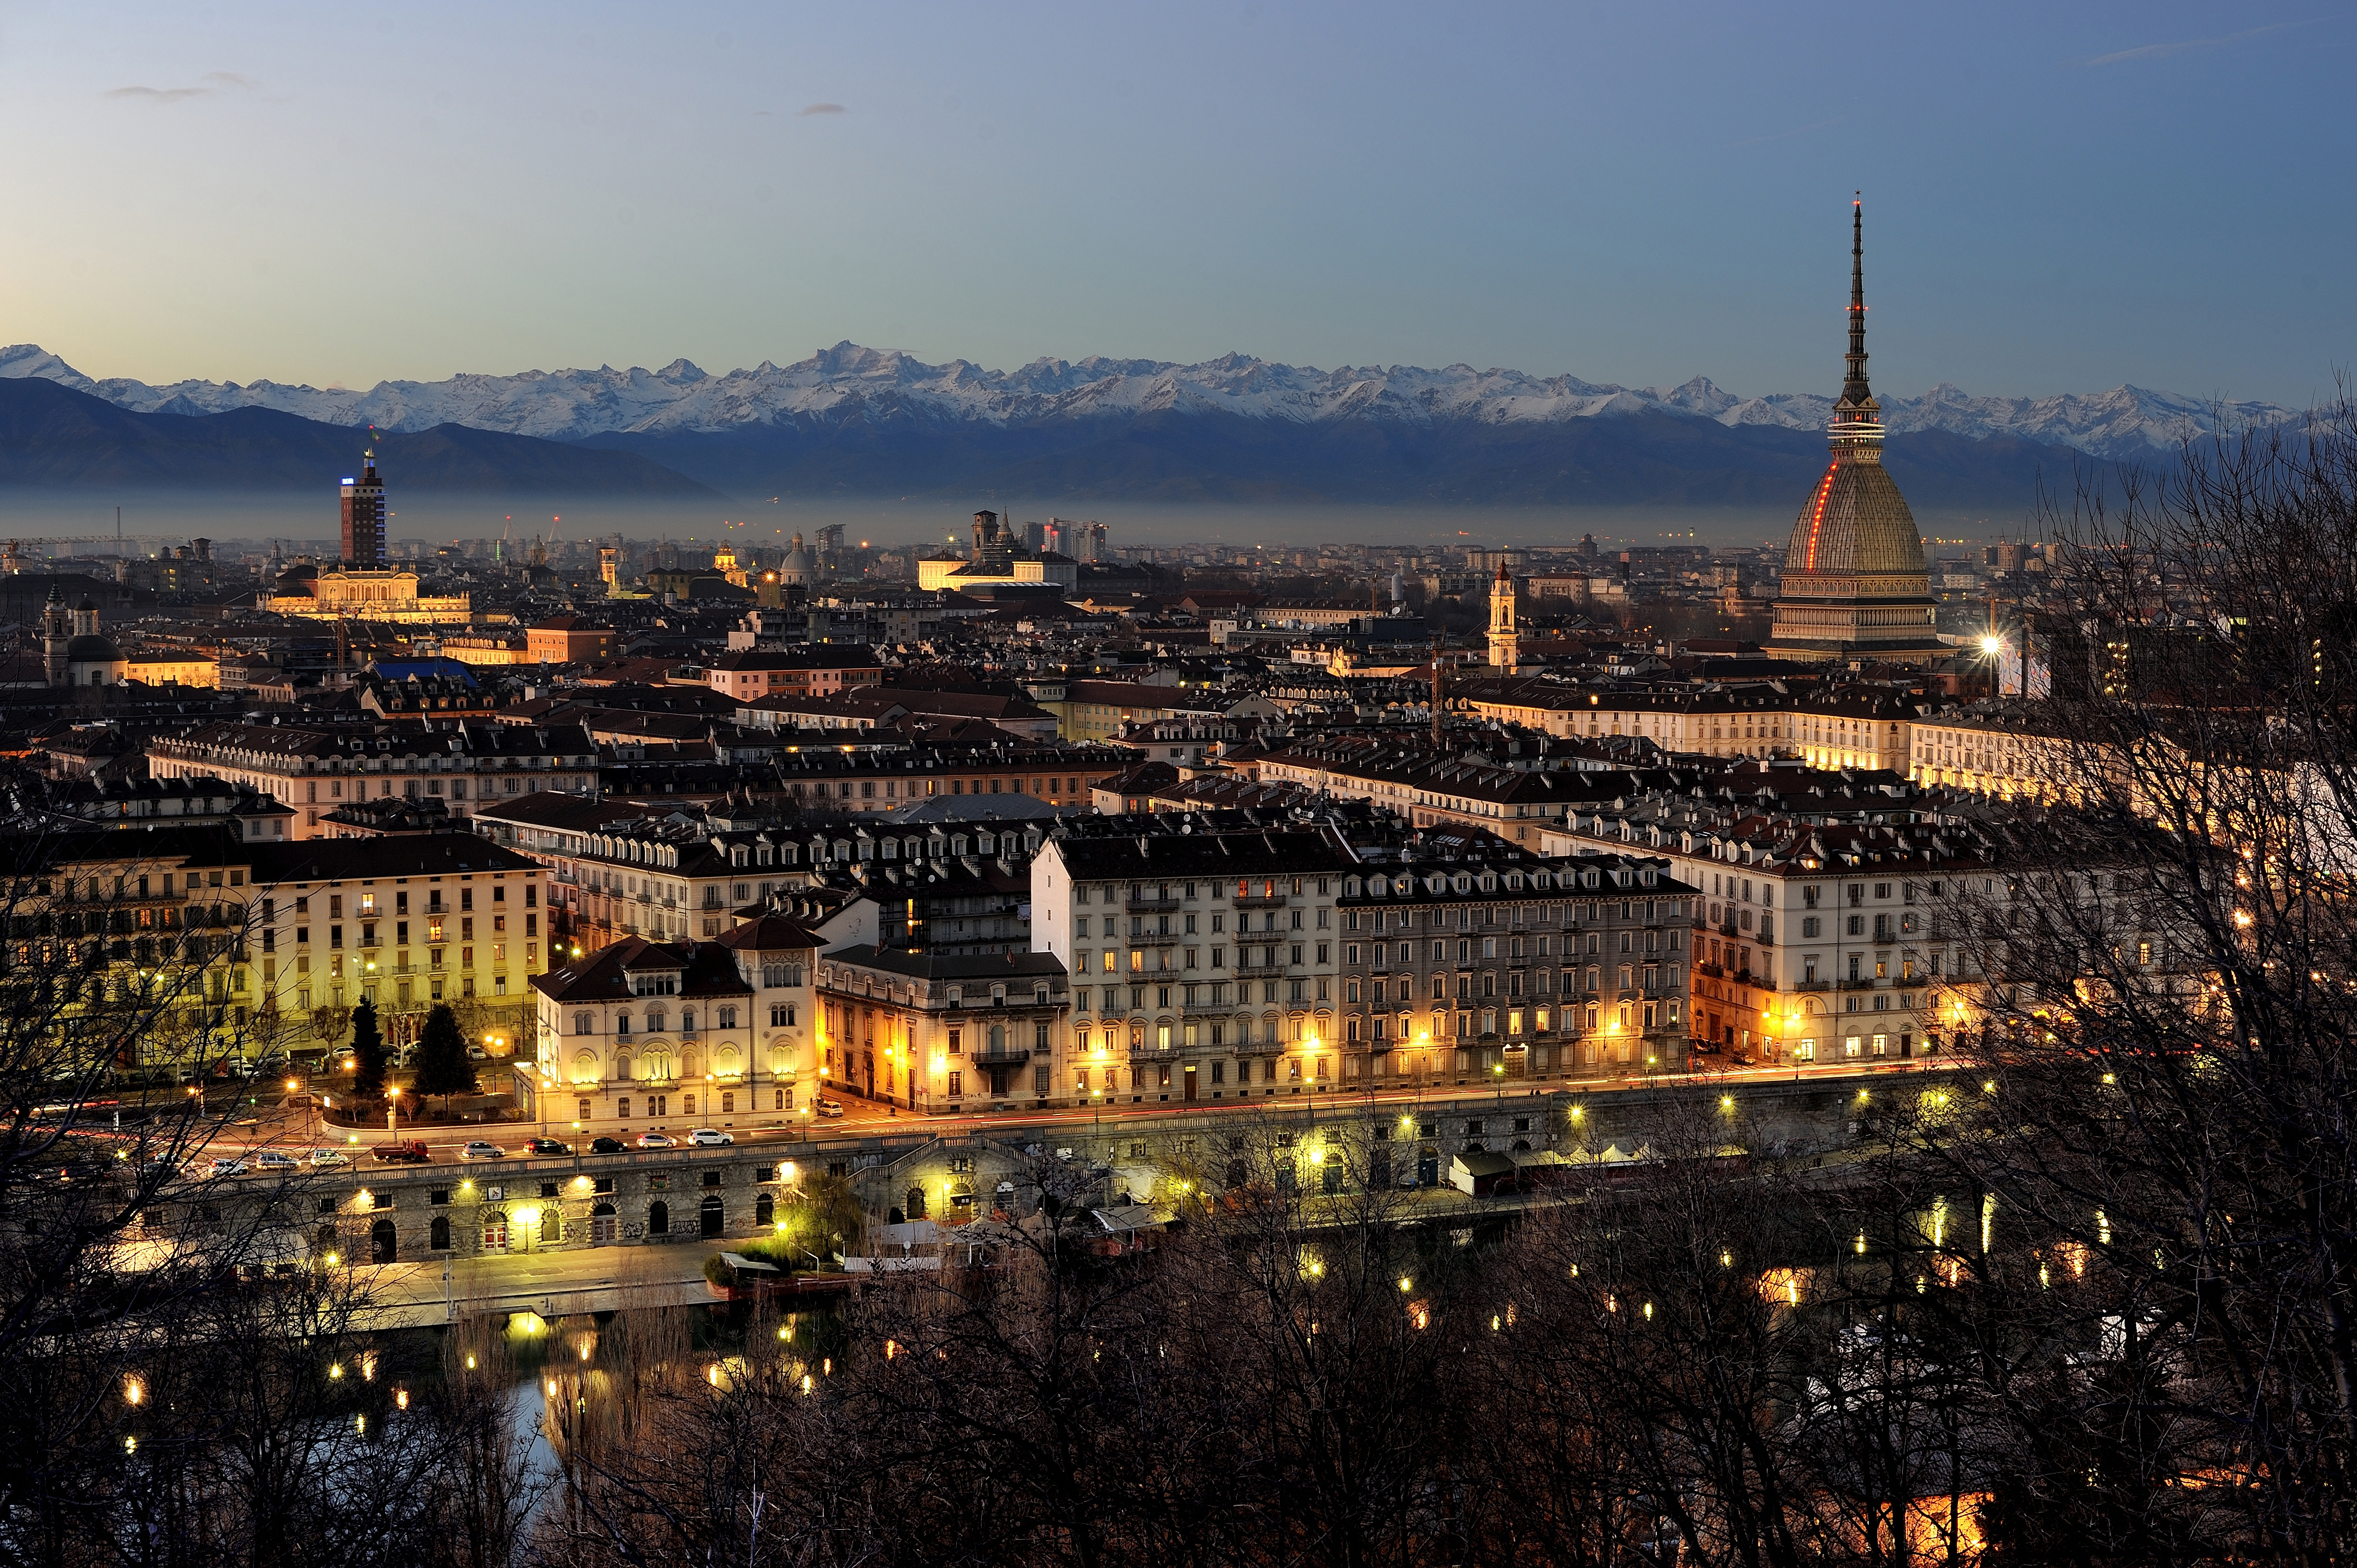
\includegraphics[scale=.5]{Turin_monte_cappuccini.jpg}%
    };%
  \end{tikzpicture}
}
\makeatother

\AtBeginSection[]{
  \begin{frame}[plain]
    \usebeamertemplate{section page}
  \end{frame}
}

\renewcommand{\thefootnote}{*}

%\setbeamercovered{transparent}

\begin{document}
%
{\usebeamercolor[fg]{structure}} %
{\usebeamercolor[fg]{block title example}} %
{\usebeamercolor[fg]{block title alerted}} %
\colorlet{basic}{structure.fg} %
\colorlet{csgreen}{block title example.fg} %
\colorlet{csred}{block title alerted.fg} %
\colorlet{csorange}{csred!50!yellow}%
% 

\maketitle

\begin{frame}
  \tableofcontents
\end{frame}

\section{Symmetries of the circle}
\label{sec:sc=sc}

\begin{frame}[fragile]{$\Sc$ as a HIT}~
  {\color{basic}$\Sc$} is postulated as a type with:
  \begin{itemize}
  \item a base point {\color{basic}$\base:\Sc$},\pause
  \item a path {\color{basic}$\Sloop: \base = \base$}.\pause
  \end{itemize}

  \vfill
  
  It comes with an {\color{basic}elimination rule}: for any
  $T : \Sc \to \UU$
  \vskip 1em%
  \begin{displaymath}
    \left.%
      \begin{aligned}
        \color{basic}t &: T(\base)
        \\
        \color{basic}\ell &: \pathover t T \Sloop t
      \end{aligned}%
      \quad\pause
    \right\}
    \qquad
    \longmapsto
    \qquad
    {\color{basic}f}: \prod_{x:\Sc} T(x)
  \end{displaymath}
  \pause such that $\color{basic}f(\base) \jdeq t$ and
  $\color{basic}f (\Sloop) = \ell$.
\end{frame}

\begin{frame}{Warming-up}~%
  In particular, functions $\color{basic}\Sc\to A$ corresponds to
  \begin{itemize}
  \item a point $\color{basic}x:A$,\pause%
  \item a symmetry $\color{basic}\ell : x = x$.
  \end{itemize}

  \vfill\pause%

  Example: define $\color{basic}-\id_\Sc$ as the function
  $\Sc \to \Sc$ given by:
  \begin{itemize}[<+->]
  \item the point $\color{basic}\base:\Sc$,
  \item the symmetry $\color{basic}\inv\Sloop : \base = \base$.
  \end{itemize}
\end{frame}

\begin{frame}{Proof sketch}~
  {\bf \color{csgreen}Goal:} prove that
  \begin{displaymath}\color{basic}%
    \left( \Sc=\Sc \right) \weq \left( \Sc + \Sc \right)
  \end{displaymath}%

  \vskip 2em\pause%
  \begin{itemize}[<+->]
  \item Identify $(\Sc = \Sc)$ with $(\Sc \weq \Sc)$%
  \item Prove that
    \begin{displaymath}
      \left(\Sc \weq \Sc\right) \weq
      \conncomp{\left(\Sc\to\Sc\right)}{\id_\Sc}
      + \conncomp{\left(\Sc\to\Sc\right)}{-\id_\Sc}
    \end{displaymath}%
  \item Identify both component with $\Sc$.
  \end{itemize}
\end{frame}

\begin{frame}{$\id_\Sc \neq -\id_\Sc$}
  Suppose $p:\id_\Sc = -\id_\Sc$, and evaluate:
  \begin{displaymath}
    \begin{aligned}
      \color{basic}f(\base) &:%
      \tikz[remember picture, baseline]{%
        \node[anchor=base, rounded corners, outer sep=0,
        alt=<2>{draw=red}{draw=white}] (baseeq) {$\base = \base$};%
      }%
      \\
      \color{basic}p(\Sloop) &: \pathover {f(\base)} {} \Sloop
      {f(\base)}
    \end{aligned}
  \end{displaymath}
  \tikz[remember picture, overlay, visible on=<2>]{%
    \node[above right of=baseeq, anchor=west, popup={color=csred!20!white}] (desc)
    {$\weq \ZZ$};%
    \draw[csred, ->, rounded corners] (desc.south) |- (baseeq.east);%
  }%
  \par\pause\pause
  i.e.\
  \begin{displaymath}
    \begin{aligned}
      \color{basic}k &: \ZZ
      \\
      \color{basic}! &: \alt<4->{\color{red}}{}\inv \Sloop \Sloop^k \inv\Sloop = \Sloop^k
      \qquad\uncover<4->{\color{red}\text{\faBolt{}}}
    \end{aligned}
  \end{displaymath}
  %
  \pause\pause\vfill%
  {\bf Consequence:}
  $\color{basic}\Trunc{f = \id_\Sc} + \Trunc{f = -\id_\Sc}$ is a
  proposition for $f:\Sc \to \Sc$.
\end{frame}

\begin{frame}{Equivalences are merely $\id_\Sc$ or $-\id_\Sc$}
  Let $\color{basic}\phi:\Sc \simeq \Sc$ and prove the proposition
  $\color{basic}\Trunc{\phi = \id_\Sc} + \Trunc{\phi = -\id_\Sc}$.

  \vskip 2em\pause%
  WLOG, suppose $\phi$ is pointed:
  $\color{basic} p:\base = \phi(\base)$.%
  
  \vskip 2em\pause%
  \begin{center}
    \tikz[node distance=5em]{%
      \node (base) {$\base$};%
      \node[right of=base] (phibase) {$\phi(\base)$};%
      \draw[transform canvas={yshift=.5em}, mid arrow] (base) to
      node[above]{\footnotesize $p$} (phibase);%
      \draw[transform canvas={yshift=-.5em}, mid arrow] (phibase) to
      node[below]{\footnotesize $\inv p$} (base);%
      \draw[mid arrow, bend left, out=135, in=45, looseness=4]
      (phibase.45) to node[right]{\footnotesize $\phi(\Sloop)$}
      (phibase.-45);%
      \draw[mid arrow, bend right, out=-135, in=-45, looseness=4, red,
      visible on=<4->] (base.135) to node[left,visible
      on=<4>]{\footnotesize \color{red}$\Sloop^k$} node[left,visible
      on=<5->]{\footnotesize \color{red}$\Sloop^{\pm 1}$} (base.-135);%
    }%
  \end{center}
  \pause\pause%
  Because $\phi$ equivalence: $\inv p\phi(\Sloop)p = \Sloop^{\pm 1}$.%

  \vfill \pause%
  In other words there is $e_1:\color{basic}\phi = \id_\Sc$ or
  $e_{-1}:\color{basic}\phi = -\id_\Sc$. Then truncate.
\end{frame}

\begin{frame}{$\Sc\to \Sc$}
  \begin{displaymath}
    \left(\tikz[baseline,remember picture]{%
        \node[anchor=base,inner sep=0, outer sep=0] (SctoSc) {$\Sc \to \Sc$};%
      } \right) \pause%
    \weq \left( \sum_{x:\Sc} \tikz[baseline,remember picture]{%
        \node[anchor=base, rounded corners, alt=<3>{draw=red}{draw=white}]
        (loopx) {$x=x$};%
      } \right) \tikz[remember picture, overlay, visible on=<3>]{%
      \node[above right of=loopx, xshift=1em, yshift=3em,
      popup={color=csred!30!white}] (label) {\footnotesize
        $\weq \ZZ$};%
      \draw[->, red, rounded corners] (label.west) -| (loopx.north);
    } \pause\pause%
    \weq \left(\tikz[baseline,remember picture]{%
        \node[anchor=base,inner sep=0, outer sep=0] (ScxZ) {$\Sc\times\ZZ$};%
    } \right)%
  \end{displaymath}
  \pause%
  \tikz[remember picture, overlay]{%
    \node[below of=SctoSc, yshift=-.5em] (id) {$\id_{\Sc}$};%
    \node[anchor=east] (-id) at ([yshift=-3em]id.east)
    {$-\id_{\Sc}$};%
    \node[below of=ScxZ, yshift=-.5em, alt=<5>{white}{}] (base1)
    {$(\base,1)$};%
    \node[anchor=west,, alt=<5>{white}{}] (base-1) at
    ([yshift=-3em]base1.west) {$(\base,-1)$};%
    \node[visible on=<5>, color=basic] at (base1) {$?$};%
    \node[visible on=<5>, color=basic] at (base-1) {$?$};%
    \draw[|->] (id) to (base1); \draw[|->] (-id) to (base-1);%
  }\pause
\end{frame}

\begin{frame}{Conclusion: $(\Sc = \Sc) \weq \Sc + \Sc$}
  \begin{displaymath}
    \left(\tikz[baseline,remember picture]{%
        \node[anchor=base,inner sep=0, outer sep=0] (SctoSc) {$\Sc = \Sc$};%
      } \right) %
    \weq  \tikz[baseline,remember picture]{%
      \node[anchor=base, rounded corners, alt=<2->{draw=csred}{draw=white}]
      (compid) {$\conncomp{\left(\Sc\to\Sc\right)}{\id_\Sc}$};%
    }  +
    \tikz[baseline,remember picture]{%
      \node[anchor=base, rounded corners, alt=<2->{draw=csred}{draw=white}]
      (comp-id) {$\conncomp{\left(\Sc\to\Sc\right)}{-\id_\Sc}$};%
    } %
  \end{displaymath}
  \pause%
  \tikz[remember picture, overlay, node distance=7em]{%
    \node[below of=compid, popup={color=csred!30!white}, alt=<3>{text
      opacity=0}{text opacity=1}] (repcompid)
    {$\conncomp{\left(\Sc\times \ZZ\right)}{(\base,1)}$};
    \node[alt=<3>{text opacity=1}{text opacity=0}] at (repcompid)
    {$\Sc$};%
    \draw[->, >={stealth},csred] (repcompid) to (compid);%
    \node[below of=comp-id, popup={color=csred!30!white}, alt=<3>{text
      opacity=0}{text opacity=1}] (repcomp-id)
    {$\conncomp{\left(\Sc\times \ZZ\right)}{(\base,-1)}$};%
    \node[alt=<3>{text opacity=1}{text opacity=0}] at (repcomp-id)
    {$\Sc$};%
    \draw[->, >={stealth},csred] (repcomp-id) to (comp-id);%
  }%
  \pause
\end{frame}

\section{Symmetries of the 2-sphere}
\label{sec:symmetries-2-sphere}

\begin{frame}{$\Sp$ as a suspension}~%
  ${\color{basic}\Sp}\defequi \susp{\Sc}$ is the suspension of $\Sc$, defined by:
  \begin{itemize}
  \item two poles $\color{basic}N,S:\Sp$,\pause
  \item for each $x:\Sc$, a path $\color{basic}\mrd(x):N=S$.
  \end{itemize}

  \vfill\pause%
  $\Sp$ comes with an {\color{basic}elimination} rule: for every
  $A:\UU$,
  \begin{displaymath}
    \left.
      \begin{aligned}
        {\color{basic} n} &: A
        \\
        {\color{basic} s} &: A
        \\
        {\color{basic} m} &: \Sc \to (n=s)
      \end{aligned}\pause\quad
    \right\}\quad
    \longmapsto
    \quad
    {\color{basic} f} : \Sp\to A
  \end{displaymath}\pause
  such that $\color{basic} f(N) \jdeq n$, $\color{basic} f(S) \jdeq s$
  and $\color{basic} f\circ\mrd = m$.
\end{frame}

\begin{frame}{Generalization}~%
  Should we expect $\color{basic} (\Sp = \Sp) \weq \Sp + \Sp$ ?\pause

  \vskip 2em%
  {\color{csred}\bf Probably not}: the argument for
  $\Sc \overset \weq \to \conncomp{(\Sc \to \Sc)}{\id_\Sc}$ relies on
  \begin{displaymath}
    {\color{basic}\loopspace {} \Sc \weq \ZZ} \qquad\text{abelian group}
  \end{displaymath}
  \pause

  \vskip 2em%
  {\color{csgreen}\bf Still plausible}: there is {\color{basic}two
    equivalent connected components}, one at $\color{basic}\id_\Sp$,
  the other at $\color{basic}-\id_\Sp$.
\end{frame}

\begin{frame}{Definition of $-\id_\Sp$}
  \begin{displaymath}
    \begin{aligned}
      \color{basic}-\id_\Sp : \Sp &\color{basic}\to \Sp\pause%
      \\
      N &\mapsto \alert{n}\defequi S\pause%
      \\
      S &\mapsto \alert{s}\defequi N\pause%
      \\
      \uncover<+(1)->{&\inv{\mrd(\blank)}} : \alert{\Sc \overset m\to S=N}
    \end{aligned}
  \end{displaymath}
  
  % \begin{displaymath}
  %   \begin{aligned}
  %     \color{basic}-\id_\Sp : \Sp &\color{basic}\to \Sp\pause%
  %     \\
  %     N &\mapsto N\pause%
  %     \\
  %     S &\mapsto S\pause%
  %     \\
  %     \uncover<+(1)->{&\mrd\circ{-\id_\Sc}} : \alert{\Sc \to N=S}
  %   \end{aligned}
  % \end{displaymath}
\end{frame}

\begin{frame}{Degree is a monoid morphism}
  The {\color{basic}degree} of a function $f:\Sp\to\Sp$ pointed by $f_0:N=f(N)$ is
  \begin{displaymath}
    \begin{tikzcd}[column sep=large,remember picture]
      |[alias=A]| {\pi_2 (\Sp)} \rar["{\pi_2(f,f_0)}"] \& \pi_2 (\Sp)
      \\
      |[visible on=<4->]| \ZZ \uar[-,"\simeq"{rotate=90,above}, visible on=<4->]
      \& |[visible on=<4->]| \ZZ \uar[-,"\simeq"{rotate=90,above}, visible on=<4->]
      \\
      |[visible on=<5->]| 1 \rar[|->, visible on=<5->] \& |[visible on=<5->]| \color{basic}d(f,f_0)
    \end{tikzcd}
  \end{displaymath}
  \tikz[remember picture, overlay, visible on=<1-3>] {%
    \node[visible on=<2->,popup={color=csred!20!white}, anchor=north east, xshift=-1em] (B) at
    (A.north west)
    {%
      \begin{minipage}[t]{.22\linewidth}
        \footnotesize$\pi_n(X) \defequi \Trunc{\loopspace n (X)}$
      \end{minipage}
    };%
    \node[visible on=<3->,popup={color=csred!20!white}, below of=B, anchor=north] (C)
    {%
      \begin{minipage}{.22\linewidth}
        \vskip -10pt\footnotesize
        \begin{align*}
          \loopspace{} X &\defequi \pt_X=\pt_X
          \\
          \loopspace {n+1} X &\defequi \loopspace{}(\loopspace n X)
        \end{align*}
      \end{minipage}%
    };%
    \draw[visible on=<3->,csred, ->, rounded corners] (C.north) to ([yshift=6pt]
    C.north) -| ([xshift=10pt] B.south);%
    \draw[visible on=<2->,csred, ->, rounded corners] (B.north) |- ([yshift=10pt]
    A.north) -- (A.north);%
  }%
    
  \vskip 2em%
  \uncover<6->{%
    Because $\pi_2$ is a functor:
    $\color{basic}d(\tikz[remember picture,baseline]{\node[anchor=base,
      alt=<7>{draw=csred}{draw=white}, rounded corners, outer sep=0] (comp) {$(g,g_0)\circ
        (f,f_0)$};}) = d(g,g_0)\times d(f,f_0)$
    \tikz[remember picture,overlay, visible on=<7>]{%
      \node[popup={color=csred!20!white}] (desc) at
      ([xshift=1em,yshift=-2em]comp.south east) {\footnotesize
        $= \left(g\circ f, g(f_0)\cdot g_0\right)$};%
      \draw[->, >={stealth}, csred, rounded corners] (desc.west) -| (comp.south);%
    }%
  }

  \vfill%
  \uncover<8->{%
    {\bf Consequence:} the degree maps pointed
    {\color{basic}equivalences} to either $1$ or $-1$.%
  }
\end{frame}

\begin{frame}{Alternative description}
  \begin{displaymath}
    \begin{tikzcd}[column sep=large]
      (\Sp \ptdto \Sp) \ar[rrr,"d",rounded corners,visible on=<14->,to path={ --
        ([yshift=10pt] \tikztostart.north) -| (\tikztotarget) [near
        start,above]\tikztonodes}]
      \rar["\susp{}\dashv\loopspace{}{}"{visible
        on=<2->},"\weq"{swap,visible on=<2->}] \& (\Sc \ptdto
      \loopspace{} \Sp) \rar["\Sc\text{-UMP}"{visible
        on=<3->},"\weq"{swap,visible on=<3->}] \& \loopspace 2 \Sp
      \rar["\color{basic}?"{visible on=<4-12>},
      "\color{basic}\loopspace{}(\tau)"{visible on=<13->}] \&
      \loopspace {}\Sc \weq \ZZ
    \end{tikzcd}
  \end{displaymath}

  \vskip 2em%
  \pause\pause\pause\pause%
  Recall the {\color{basic}Hopf family}:
  \begin{displaymath}
    \begin{aligned}
      \color{basic} \hopffam : \Sp &\color{basic}\to \UU\pause%
      \\
      N &\mapsto \alert{n}\defequi\Sc\pause%
      \\
      S &\mapsto \alert{s}\defequi\Sc\pause%
      \\
      x&\mapsto \tikz[remember picture, baseline]{%
        \node[anchor=base, outer sep=0, alt=<9-12>{draw=red}{draw=white},
        rounded corners] (equi) {$(x,\Sloop_x)$};%
      } : \alert{\Sc \overset m \to (\Sc=\Sc)}
    \end{aligned}
  \end{displaymath}
  \tikz[remember picture, overlay, visible on=<9-12>]{
    \node[popup={color=csred!20!white}] (defequi) at ([xshift=13em, yshift=5em] equi) {
      \begin{minipage}[t]{.4\linewidth}
        \vskip -10pt\footnotesize
        \begin{align*}
          \base &\mapsto x
          \\
          \Sloop &\mapsto \uncover<12->{\Sloop_x} : (x=x) \uncover<10->{\weq (\base=\base)}
                   \uncover<11>{: \Sloop}
        \end{align*}
      \end{minipage}
    };%
    \draw[csred, rounded corners, ->] (defequi.west) -|
    ([xshift=10pt,yshift=-3pt] equi.north east) to
    ([yshift=-3pt]equi.north east);%
  }

  \vskip 2em%
  \pause\pause\pause\pause\pause
  Define $\color{basic}\tau(p) \defequi \trp[\hopffam] p(\base)$ for $p:N = N$.
\end{frame}

\begin{frame}{Alternative description (cnt'd)}
  \begin{displaymath}
    \begin{tikzcd}[column sep=large, remember picture]%
      (\Sp \ptdto \Sp) \ar[rrr,"d",rounded corners,to path={ --
        ([yshift=10pt] \tikztostart.north) -| (\tikztotarget) [near
        start,above]\tikztonodes}]
      \rar["\susp{}\dashv\loopspace{}{}","\weq"{swap}] \& (\Sc \ptdto
      \loopspace{} \Sp) \rar["\Sc\text{-UMP}","\weq"{swap}] \&
      \loopspace 2 \Sp
      \rar["\color{basic}\loopspace{}(\tau)"{name=trunc}] \&
      \loopspace {}\Sc \weq \ZZ
    \end{tikzcd}
  \end{displaymath}
  \tikz[remember picture, overlay, visible on=<2->]{%
    \node[text=csred, anchor=east] (desc) at
    ([xshift=-2em,yshift=-4em] trunc) {\footnotesize Set truncation
      map};%
    \draw[csred, ->, rounded corners] (desc.east) -| ([yshift=-.5em] trunc.south);
  }%

  \pause\pause
  \vskip 4em%
  {\bf \color{csgreen}Consequence:} for
  $(f,f_0), (g,g_0) : \Sp \ptdto \Sp$,
  \begin{displaymath}
    {\color{basic}d(f,f_0)=d(g,g_0)} \iff {\color{basic}\Trunc{(f,f_0)=(g,g_0)}}.
  \end{displaymath}
\end{frame}

\begin{frame}{Putting things together}
  As in the case of $\Sc$, one can prove $\id_\Sp \neq -\id_\Sp$.

  \vskip 2em\pause%
  Hence, proving $\color{basic}\Trunc{f = \id_\Sp} + \Trunc{f = -\id_\Sp}$ for an
  equivalence $\color{basic}f:\Sp \weq \Sp$, one can suppose that $f$ is pointed by some $f_0:N=f(N)$.

  \vskip 2em\pause%
  Then $\color{basic}d(f,f_0) = \pm 1$. Also, $d(\id_\Sp, \refl N) = 1$ and
  $d(\id_\Sp, \inv{\mrd(\base)}) = 1$.

  \vskip 2em\pause%
  This yield
  $\color{basic}\Trunc{(f,f_0)=(\id_\Sp,\refl
    N)}+\Trunc{(f,f_0)=(-\id_\Sp,\inv{\mrd(\base)})}$.

  \vskip 2em\pause%
  Proving that both component are equivalent is easy. QED.
\end{frame}

\section{Symmetries of higher spheres}
\label{sec:symm-high-spher}

\begin{frame}{Sketch of the proof}
  Inductively, $\color{basic}\Sn {n+1} \defequi \susp{\Sn n}$ with the
  appropriate {\color{basic}elimination rule}.

  \pause%
  {\color{csgreen} \bf Goal:} prove for all $n:\mathbb N$ that
  $\color{basic}(\Sn n = \Sn n)$ has two equivalent connected
  components, one centered at $\id$, the other one centered at $-\id$.

  \pause%
  \begin{itemize}
  \item The case $n=0$ is almost immediate. The case $n=1$ has been
    treated.  The case $n=2$ has been treated and is the base
    case.\pause%
  \item Inductively, prove that
    \begin{displaymath}\color{basic}%
      \Trunc{\Sn n \ptdto \Sn n}_0 \xrightarrow{\Trunc{\Sigma\blank}_0}
      \Trunc{\Sn {n+1} \ptdto \Sn {n+1}}_0 
    \end{displaymath}
    is an equivalence of monoids for every $n\geq 2$. (Using Freudenthal
    suspension theorem.) \pause%
  \item Conclude that $\Trunc{(\Sn n, N) \weq_\ast (\Sn n ,x)}_0$ is {\em
      merely} equivalent to $\bool$ for any $x:\Sn n$.\pause%
  \item Derive that $\color{basic}\Trunc{\Sn n \weq \Sn n}_0$ is {\em
      merely} equivalent to $\color{basic}\bool$.\pause%
  \item Get rid of the ``{\em merely}'' in the above statement.
  \end{itemize}
\end{frame}

\end{document}
